\documentclass{article}
\usepackage{bera}
\usepackage{float}
\usepackage[margin=1in]{geometry}
\usepackage{graphicx}

\usepackage[colorlinks=true,linkcolor=blue,citecolor=yellow,filecolor=magenta,urlcolor=cyan]{hyperref}
\newcommand{\cymisversion}{0.1}
\title{SDMM v\cymisversion\space User Guide}
\author{Pherakki}
\date{}

\begin{document}
\maketitle

\tableofcontents
\clearpage
\pagenumbering{arabic} 
\section{Introduction}
\subsection{Overview}
SimpleDSCSModManager (SDMM) is a poorly-named mod manager and mod-merging utility designed for the PC release of Digimon Story Cyber Sleuth: Complete Edition (DSCS). It is relatively straightforward program for an end-user to use, with a drag-and-drop graphical user interface. SDMM takes a list of mods, and patches them together into a set of asset files that can then be injected into the game data. This approach is taken due to the way that DSCS loads assets, and is the reason for much of the complexity behind SDMM. Mod authors are responsible for using the tools that SDMM gives them for making their mods as compatible as possible with other mods, although the list of tools that SDMM will provide will grow as time goes on.

This document is for the \textbf{v\cymisversion} release of SDMM. This means that the mod manager is still a work-in-progress, and although it should be good for many applications, it is not feature-complete and lacks certain useful functionality, and may also suffer from bugs.

\subsection{A Tour of the UI}\label{Section:UITour}
Here we'll take a look at the areas of the user interface (UI) that an end-user is likely to interact with. Later sections of this guide will re-introduce areas of the UI in-context, referring back to the definitions made in this section.

\subsubsection{Mod Activation Window}
One of the most important areas of the UI is the \textbf{Mod Activation Window}, which displays all mods currently registered with the mod manager. You will use this list to activate, add, delete, and re-configure mods known to the mod manager. You can add mods by dragging-and-dropping ZIP files onto the Mod Activation Window. Mods can be deleted by right-clicking and selecting ``Delete" on a mod. Mods that use CYMIS installers can be re-configured by selecting the ``re-register" option in the right-click menu.

\textbf{The order of mods defines the install order.} You can re-arrange these mods by dragging-and-dropping mods inside this window.
\begin{center}
  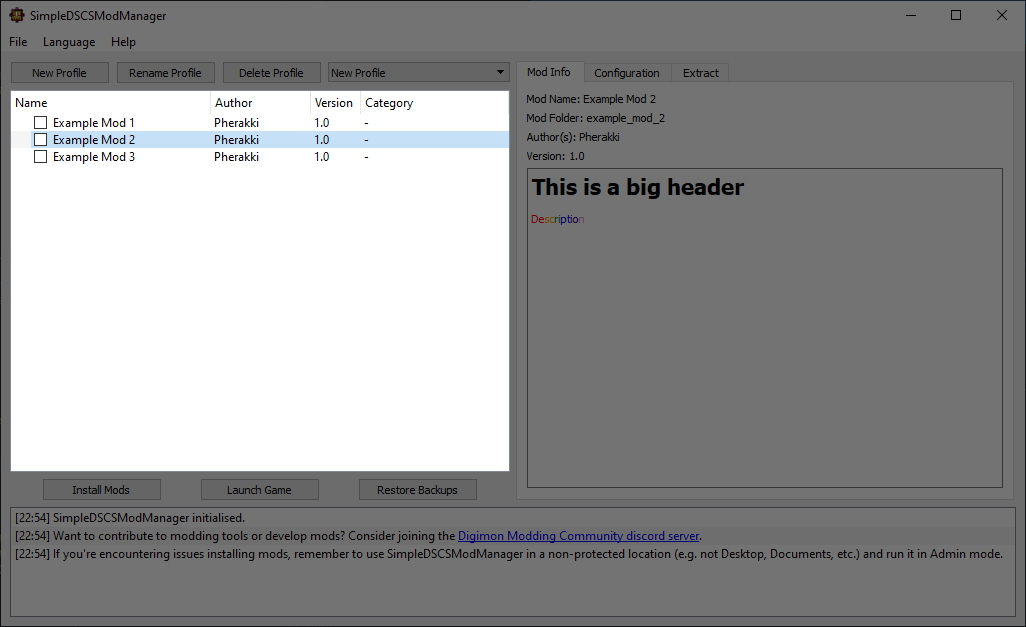
\includegraphics[scale=0.4]{img/modmanager_ui_modslist.jpg}
\end{center}
\newpage
\subsubsection{Mods Interaction Buttons}
Use these three buttons to manage what game data is currently installed. The ``Install Mods" button will initiate a patching process that combines all activated mods together, adds them to the vanilla files, and then injects them into the game data. ``Launch Game" is a shortcut for launching the game, and it is not required to use this button for mods to work. ``Restore Backups" will uninstall all mods and restore the game to a vanilla state.
\begin{center}
  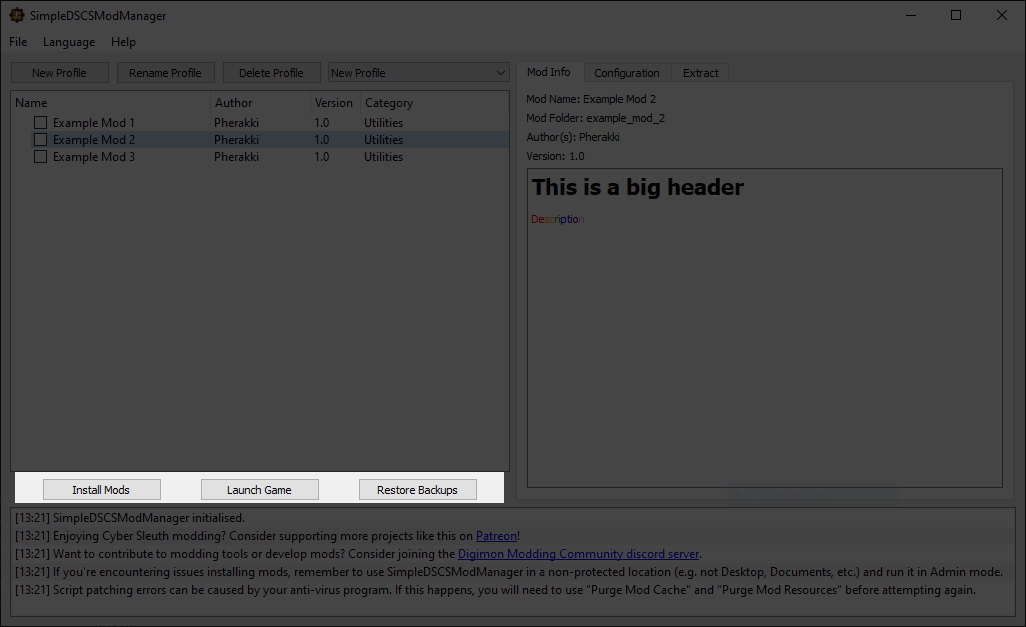
\includegraphics[scale=0.4]{img/modmanager_ui_modinteractionbuttons.jpg}
\end{center}

\subsubsection{Log}
The log displays important messages and keeps you informed about what the mod manager is currently doing, as well as any errors that may occur.
\begin{center}
  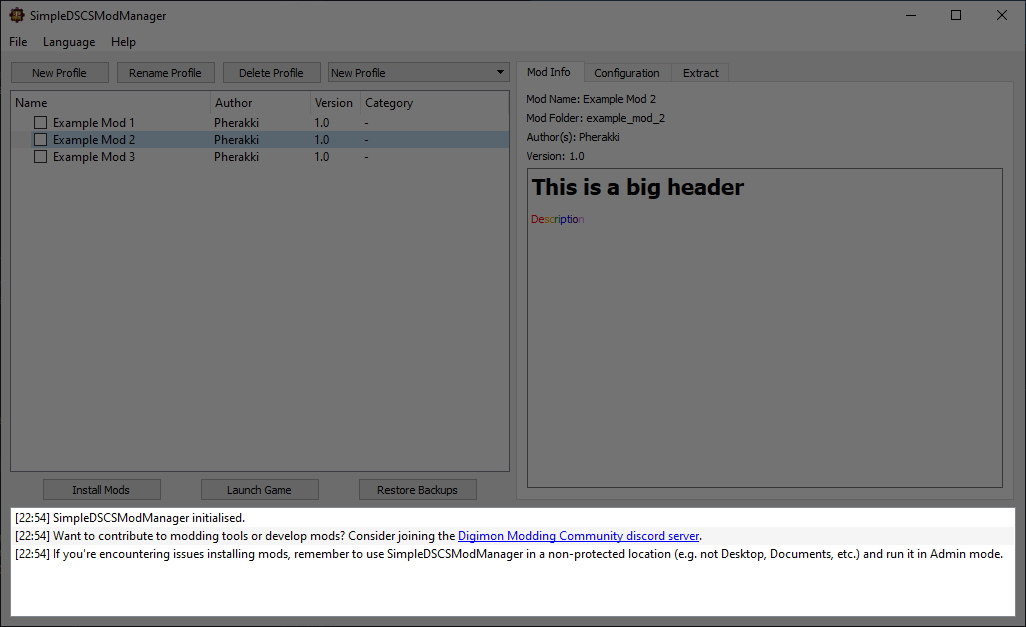
\includegraphics[scale=0.4]{img/modmanager_ui_log.jpg}
\end{center}
\newpage
\subsubsection{Information Tabs}
These tabs switch between different information and action displays on the right-hand side of the manager.\begin{center}
  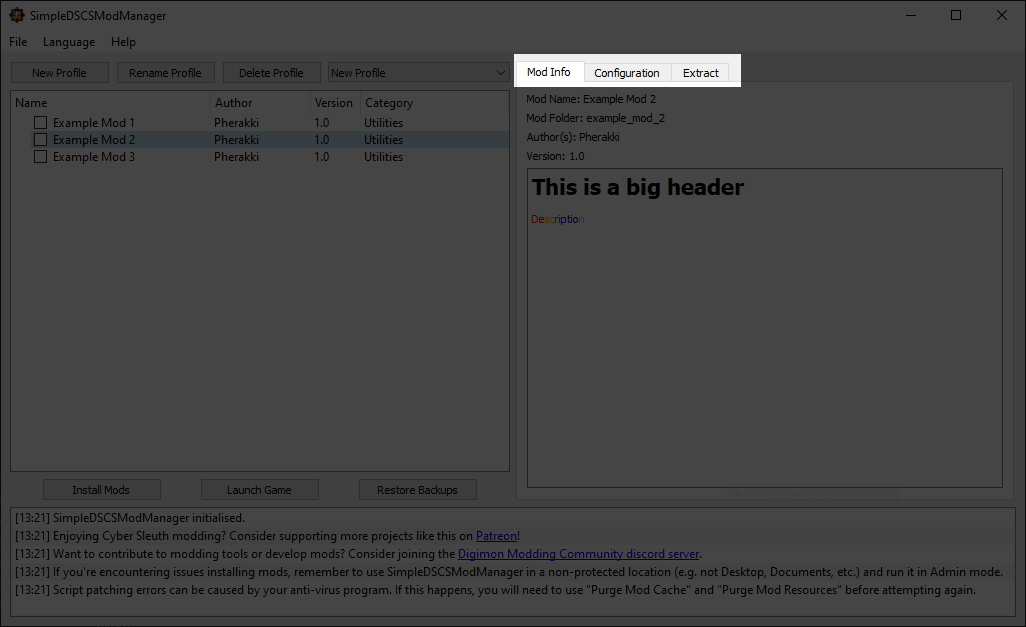
\includegraphics[scale=0.4]{img/modmanager_ui_infotabs.jpg}
\end{center}

\subsubsection{Mod Information Tab}
The Mod Information Tab displays details about the currently selected mod, including an HTML-rendered description.
\begin{center}
  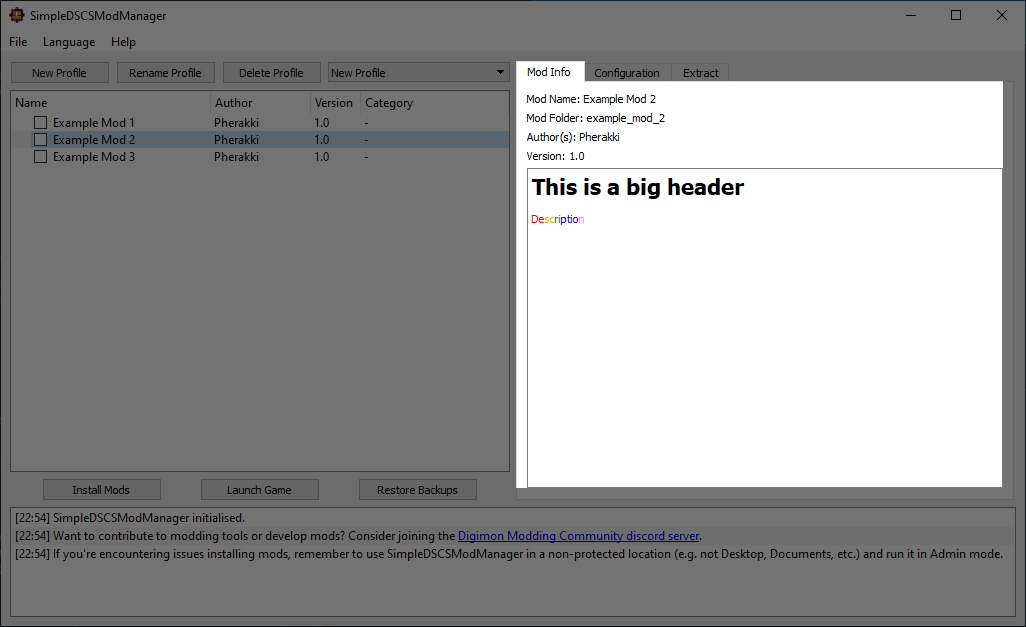
\includegraphics[scale=0.4]{img/modmanager_ui_modinfo.jpg}
\end{center}

\newpage


\subsubsection{Manager Configuration Tab}
The Configuration Tab provides a number of important functions to alter the way the mod manager behaves, and to repair broken functionality.
\begin{itemize}

\item The ``Game Location" box allows you to select your game location if the mod manager has mistakenly loaded the wrong path. 

\item The ``Purge Softcodes" button should be ignored by a general user for now, because using it will probably break your savegames. It is used to wipe any stored cached ``Softcodes" used by the mod manager to auto-assign IDs to game data records.  If you reach the Softcode cap, you'll need to use this button eventually, but that is somewhat unlikely.

\item ``Purge Mod Indices" can also probably be ignored by a user, since this is used to clear registry files generated by the mod manager for each mod that accelerates their install times. The button exists in case these files fail to update when mod data is changed. 

\item ``Purge Mod Cache" is used to delete saved assets previously built by the mod manager to speed up installation times. This button can be used in the case that these assets have been built incorrectly. 

\item The ``Purge Mod Resources" button deletes a cache of extracted vanilla game files used during the patching process. This button can be used if those resources have been extracted incorrectly.

\item The ``Crash Method" is how the mod manager will respond to errors. ``UI" will attempt to print a log message, ``Crash+Log" will cause a CTD and generate a log file that you can upload as part of an issue. 

\item ``Game Launch Method" tells the mod manager how to behave when you click the ``Launch Game" button. ``Popup" will block the mod manager from being interacted with by launching a popup. ``Quit" will close the mod manager when you launch the game from the manager.
\end{itemize}
\begin{center}
  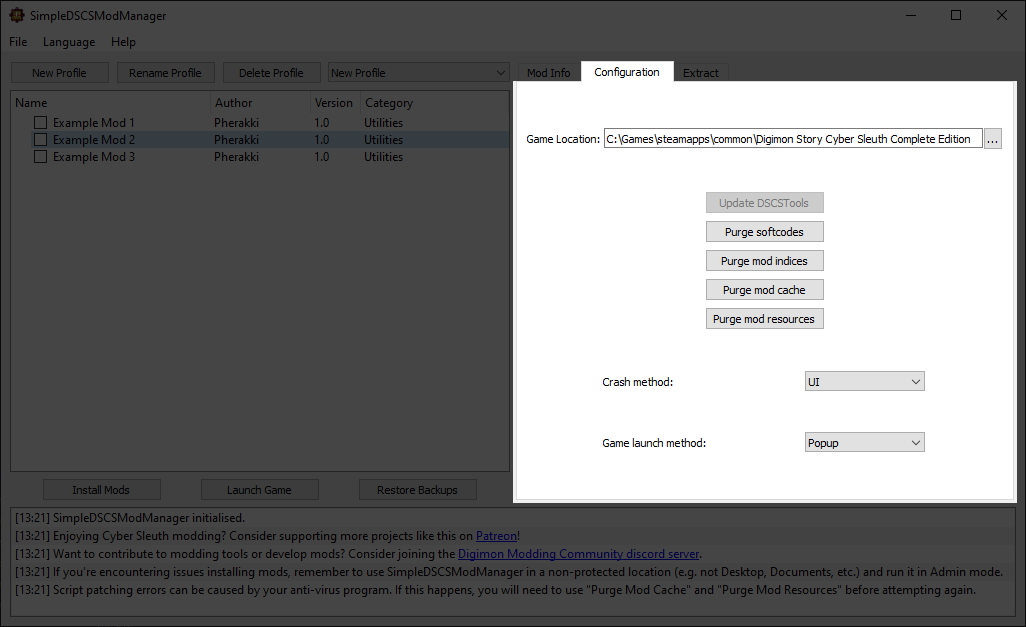
\includegraphics[scale=0.4]{img/modmanager_ui_config.jpg}
\end{center}
\newpage

\subsubsection{Profile Interaction Buttons}
The mod manager has a ``profile" feature which allows you to save certain sets of activated mods to switch between. These four widgets allow you to manage profiles; creating, renaming, deleting, and selecting profiles. Note that at least one profile must exist at all times.
\begin{center}
  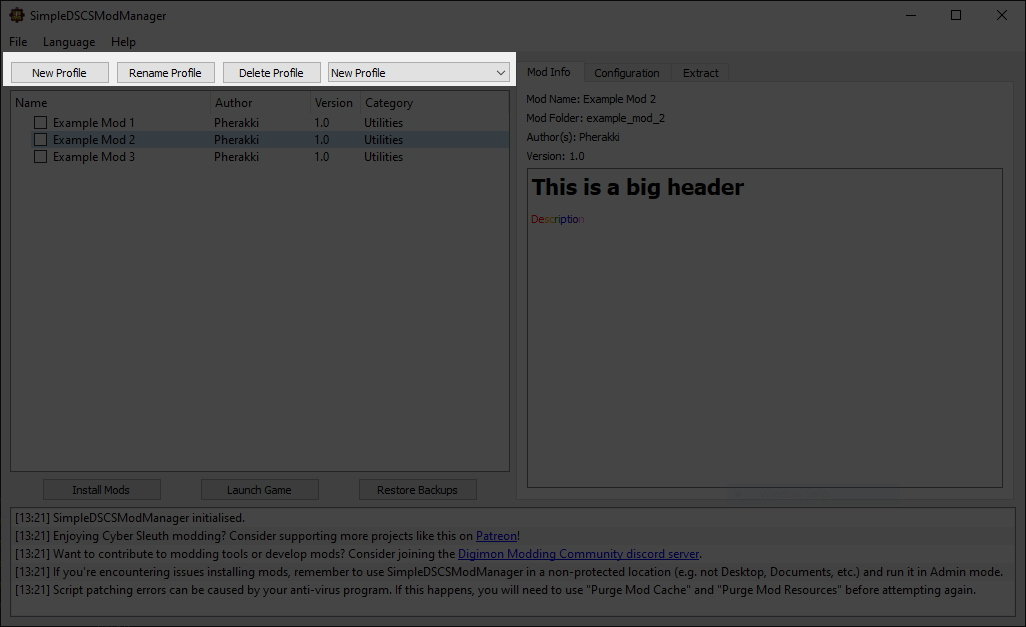
\includegraphics[scale=0.4]{img/modmanager_ui_profileinteraction.jpg}
\end{center}


\subsubsection{File Menu}
The File menu contains a single option, which is to add a mod. You can select a ZIP file that contains a mod in order to add a mod in this method. The alternative is to drag-and-drop zip files into the Mod Activation Window.
\begin{center}
  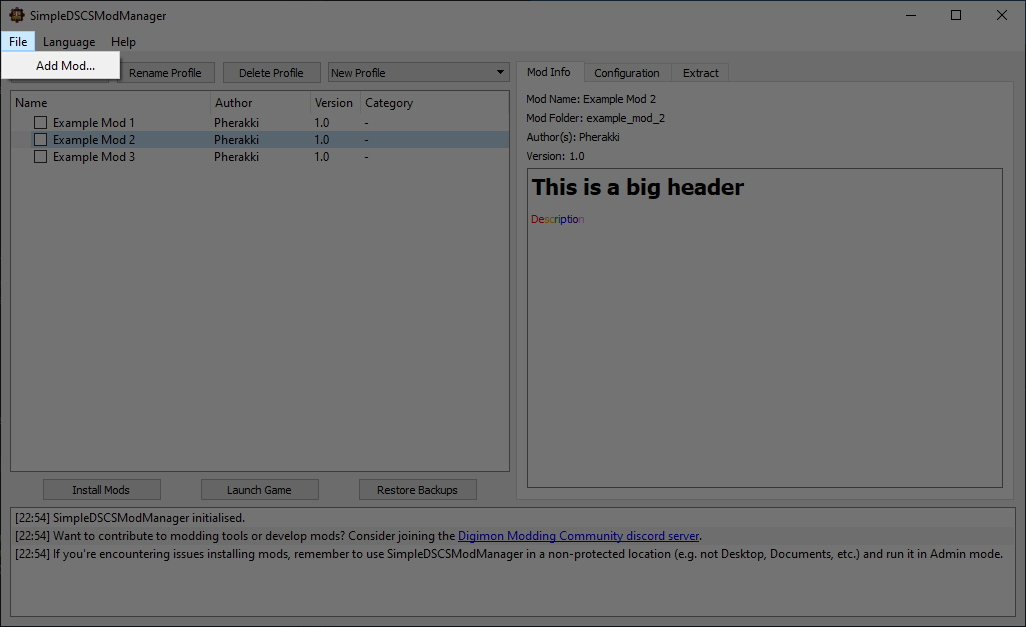
\includegraphics[scale=0.4]{img/modmanager_ui_filemenu.jpg}
\end{center}

\newpage

\subsubsection{Language Menu}
The Language menu allows you to switch between different localisations of the mod manager.
\begin{center}
  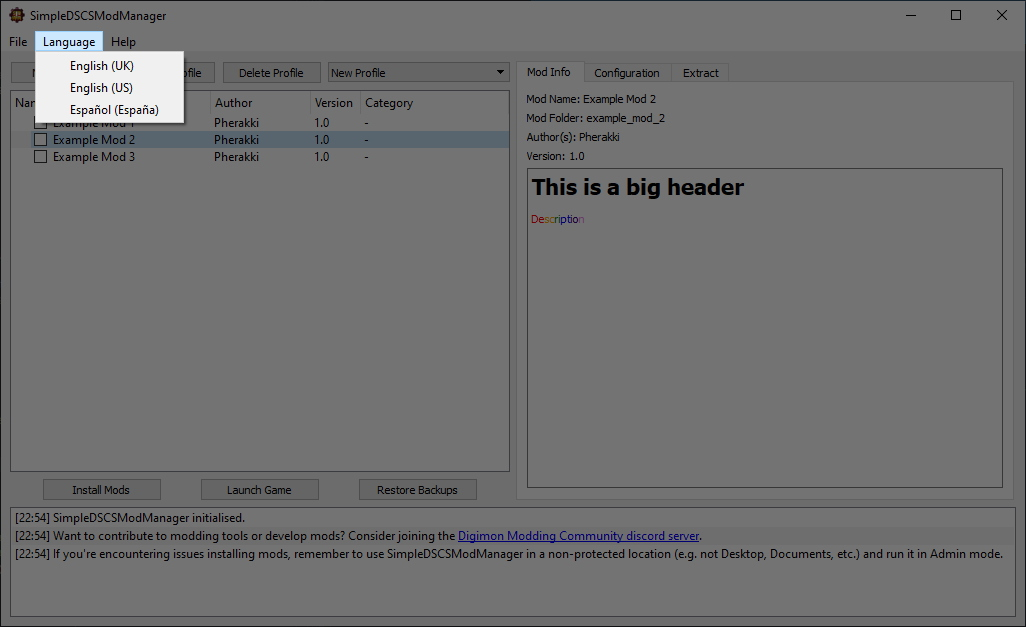
\includegraphics[scale=0.4]{img/modmanager_ui_languagemenu.jpg}
\end{center}

\subsubsection{Help Menu}
The Help menu currently does not contain any links to documentation; but does contain links to SydMontague's Patreon and credits for the mod manager.
\begin{center}
  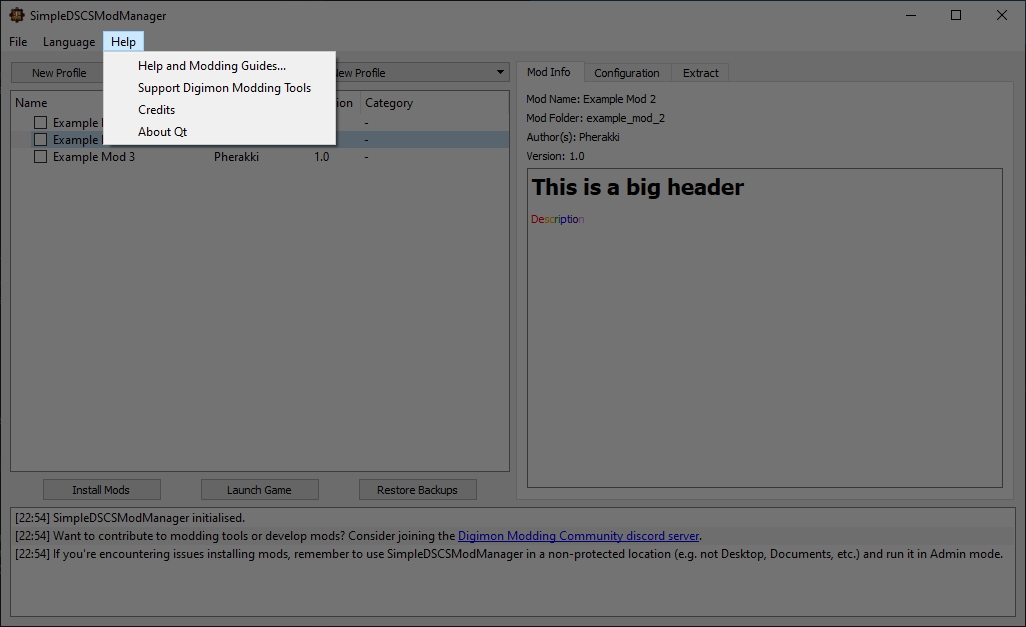
\includegraphics[scale=0.4]{img/modmanager_ui_help.jpg}
\end{center}
\newpage


\section{Using the Manager to Install Mods}
\subsection{Overview}
The mod manager is relatively simple to use if you want to install mods. There are three main stages to mod installation:
\begin{enumerate}
\item Registering mods in the manager.
\item Activating registered mods.
\item Installing mods to the game archive.
\end{enumerate}
We'll go through each of these three steps in the following sections. It's a good idea to familiarise yourself with the UI, which is reproduced below, by reading through section \ref{Section:UITour}.

  \begin{center}
    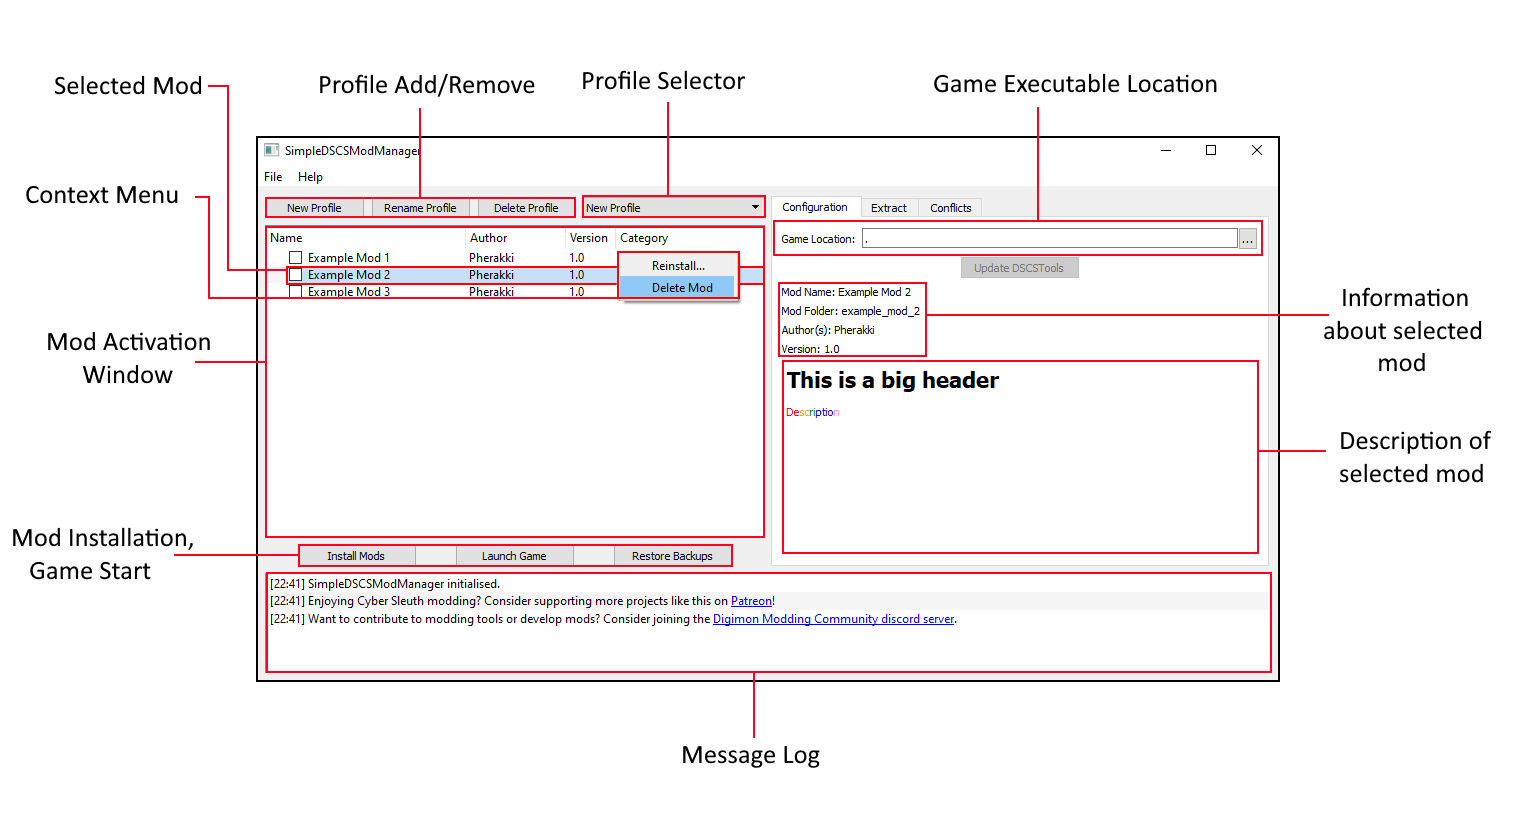
\includegraphics[scale=0.406]{img/modmanager_ui.png}
  \end{center}
  
\subsection{A Note on Savegames}
Before beginning, you should \textbf{make a backup of your savegames}. Modding always carries the risk of breaking savegames. Your savegames are located at 
\begin{center}
\textbf{\%localappdata\%\textbackslash BANDAI NAMCO Entertainment\textbackslash Digimon Story Cyber Sleuth Complete Edition\textbackslash Saved\textbackslash SaveGames}
\end{center}
inside the single folder in this directory. The savegame files are 
\begin{itemize}
\item 0000.bin
\item 0001.bin
\item 0002.bin
\item slot\_0000.bin
\item slot\_0001.bin
\item slot\_0002.bin
\item system\_data.bin
\end{itemize}
You should back up these saves and keep a copy for each set of mods you install. Future version of the mod manager will include automatic savegame management. The safest way to mod is to start a new game. \textbf{Do not remove mods that add new data from a saved game}.
  
\subsection{Registering Mods}
Registering a mod with the manager allows the manager to install the mod into the game files.\\
Registered mods are displayed in the \textbf{Mod Activation Window}.\\\\
There are two ways to register a mod with the manager. The first is to open \textbf{"File > Add Mod..."} in the toolbar, which will open a file dialog. A mod contained in a zip archive an then be selected from this file dialog.\\
The second and arguably simpler way is to drag-and-drop the mod into the \textbf{Mod Activation Window}. Any supported mod format can be installed this way, including an unarchived folder in the correct mod format.
If the mod uses a CYMIS installer, you will be prompted to select what install options you want. It is possible to re-install such a mod with different options \textit{via} the right-click \textbf{context menu}.\\\\
If you ever want to unregister a mod, you can delete the files from the mod manager \textit{via} the right-click \textbf{context menu}.

\subsection{Activating Mods with Profiles}
This mod manager makes use of a \textbf{profile} system to allow different combinations of mods to be installed. You can switch between profiles by clicking the \textbf{profile selector}, which will display all the profiles you have created.\\
You can add, rename, and remove profiles by using the buttons to the left of the \textbf{profile selector}. Note that at least one profile must always be present, and the mod manager will prevent you from deleting the final profile.\\
To select which mods are to be installed by the \textbf{profile}, click the checkboxes next to the mod names. If it is checked, it will be installed during the next step.\\
If you click on a mod in the \textbf{Mod Activation Window}, then metadata about that mod will be displayed in the \textbf{"Configuration"} tab on the right-hand side of the manager. This will summarise the name of the mod, the name of the folder it is registered in in the manager files, the version, and category. Below these data, there is also a space to render a mod description in HTML.

\subsection{Installing Mods}
This is by far the simplest step for the user, but also the place where things are most likely to go wrong. Now that you have activated some mods, click the "Install Mods" button below the \textbf{Mod Activation Window}. This will begin the process of patching your selected mods together, and installing them into the game files. Depending on the number and size of the mods that are active, this can take several minutes to complete.\\
The adjacent button will launch the game, for convenience.\\
If you ever want to restore the game to a vanilla state, click the "Restore Backups" button, which is located to the right of the "Launch Game" button.

\newpage
\section{Troubleshooting and FAQ}
\subsection{The mod manager crashes when it's packing the archive!}
This is an unknown bug that occasionally causes the mod manager to hang when it is packing archives. This strikes randomly; just close the mod manager and attempt installation again.

\subsection{The mod manager keeps giving me errors halfway through installation!}
There are three likely causes of this, enumerated below. If the mod manager crashes during installation, there is the possibility that the mod manager caches get poisoned with corrupt data. It is therefore a good idea to use the \textbf{Purge Mod Cache} and \textbf{Purge Mod Resources} buttons to clear these caches if you encounter issues.
\begin{enumerate}
\item In 99\% of cases, it is because you are using the mod manager from a protected location in Windows. Windows loves to interfere with and break programs running in certain places, such as Desktop, Documents, or Program Files. You should receive a popup when opening the mod manager warning you not to do this. \textbf{Do not ignore it.} Move the mod manager to an unprotected location, and run it in admin mode.
\item During alpha development, some problems were noticed with anti-virus software such as Avast interfering with the vanilla file extraction process. This may have been due to the game being installed in Program Files. These issues seem to have been resolved, but this cannot be guaranteed. \textbf{Only use an official release of SimpleDSCSModManager and do not disable your anti-virus if you are running a copy not downloaded from GitHub or GameBanana}.
\item You are installing a buggy mod.
\end{enumerate}
\subsection{The mods I'm installing aren't behaving properly!}
Follow the advice given in the above question. As a first check, clear the cache and resources and check if that fixes the issue. Failing that, ensure that the mod manager and the game are both outside of protected locations, as you should do when modding most games.
\subsection{Why do I get a log error during the archive-building step when I have lots of mods?}
DSCS uses 32-bit addresses in its asset archive format. This means that an archive cannot contain more than 4~GiB of compressed data. If you have many mods, or have mods that introduce a lot of data, you may hit this 4~GiB limit. Currently, the only way around this issue is to install game data into multiple archives with free space, of which there are 4, meaning we can theoretically install $\sim$16~GiB of new asset data. However, the mod manager is currently only set up to install all data into a single 4~GiB archive unless it is told otherwise. The 16~GiB hack is one option to increase the amount of space available for mods, and there are also other ideas being considered.

\subsection{How do I report a bug?}
The best way is to submit an issue to the \href{https://github.com/Pherakki/SimpleDSCSModManager/issues?q=is\%3Aopen+is\%3Aissue}{issue tracker}. This requires a GitHub account. Please collect as much information as possible to assist with tracking down the issue, including the crash log generated by the mod manager. Issues with very little information will likely be closed due to being impossible to debug. Bugs can also be reported in the Digimon Modding Community.
 
\subsection{Can I contribute to SDMM?}
Yes. The most significant form of help is Python and (in the future) C++ developers who wish to add features to SDMM or port features to C++, since at the time of writing SDMM has been programmed by a single developer with many projects to juggle. You can also provide translations of the mod manager if you are familiar with Qt Linguist and Qt translation files. Feel free to contact me \textit{via} the contact details given in the SDMM repository, or in the Digimon Modding Community Discord server.
\end{document}